\section{Experimental Results}
\label{sec:results}

In this section, we present a qualitative evaluation of our LLM-based psychological counseling agent and its WeChat Mini Program frontend. While the FAITA-MENTAL framework\cite{golden2024describing} provides a comprehensive set of evaluation domains for LLMs in mental health applications, it does not offer a ready-to-use dataset or benchmark for direct quantitative assessment. Moreover, the primary scope of our project is to design a robust workflow for applying LLMs in psychological counseling, rather than optimizing for benchmark performance. As LLM technology advances, our agent can naturally benefit from future improvements.

\subsection{Settings}

Our system consists of a backend agent implemented with a modular, workflow-driven architecture (see Section~\ref{sec:methodology} Methodology), and a WeChat Mini Program as the user interface. The agent leverages large language models(LLM configuration see Appendix~\ref{sec:manual} Manual) for dialogue, mood analysis, and event extraction.

\subsection{FAITA-MENTAL Evaluation Framework}

The FAITA-MENTAL framework defines 12 key domains for evaluating LLM-based mental health system. Table~\ref{tab:faita-mental} summarizes the coverage of each domain in our system, where \checkmark~indicates the domain is addressed, and \xmark~indicates it is not fully covered.

% Table: FAITA-MENTAL Domain Coverage

\begin{table}[h]
\centering
\begin{tabular}{lcc}
\toprule
\textbf{FAITA-MENTAL Domain} & \textbf{Introspection Agent} \\
\midrule
Proposed goal & \checkmark \\
Evidence-based content & \checkmark \\
Retention & \checkmark \\
Personalization and evolution & \checkmark \\
Interactivity quality & \checkmark \\
Feedback mechanism and support & \checkmark \\
User autonomy, data protection, and privacy & \xmark \\
User empowerment & \xmark \\
Cultural sensitivity and inclusivity & \xmark \\
Bias and fairness & \checkmark \\
Transparency & \checkmark \\
Safety and crisis management & \checkmark \\

\bottomrule
\end{tabular}
\caption{Coverage of FAITA-MENTAL domains in our system (\checkmark: addressed, \xmark: not fully addressed).}
\label{tab:faita-mental}
\end{table}

\subsection{Qualitative Analysis}

Based on the FAITA-MENTAL framework's 12 key domains, we provide a qualitative analysis of how the Introspection Agent addresses each area. For domains that are covered (\checkmark), we describe the implementation and strengths; for those not fully addressed (\xmark), we briefly discuss the limitations.

\paragraph{Addressed Domains (\checkmark)}
\begin{itemize}
    \item \textbf{Proposed goal:} The system is designed with a clear, specific, and measurable goal: to provide non-clinical, evidence-based psychological support and self-reflection tools for users, especially adolescents, via a WeChat Mini Program.
    \item \textbf{Evidence-based content:} Core features such as mood analysis and event extraction are grounded in established psychological theories (e.g., Cognitive Behavioral Therapy). The agent structures user input into interpretable psychological constructs, making evidence-based content explicit and actionable.
    \item \textbf{Retention:} The current system include medal mechanisms to track and promote long-term user engagement.
    \item \textbf{Personalization and evolution:} The agent maintains user profiles and conversation history, enabling personalized responses and adaptive dialogue strategies. User feedback on mood and event extraction results is incorporated to refine future interactions, supporting continuous improvement.
    \item \textbf{Interactivity quality:} The system delivers natural, contextually appropriate, and supportive interactions. Dialogue flows are guided by a planning module that ensures responses are empathetic and relevant to the user's current state.
    \item \textbf{Feedback mechanism and support:} Users can provide direct feedback on mood and event analysis results, including editing, confirming, or rejecting system-generated content. This human-in-the-loop mechanism ensures that the final records reflect the user's own understanding and preferences.
    \item \textbf{Bias and fairness:} The agent is designed to minimize bias by using neutral, supportive language and by allowing users to review and correct analytical outputs. The system does not make clinical diagnoses, reducing the risk of inappropriate or biased advice.
    \item \textbf{Transparency:} The development process, system architecture, and data flow are documented in the project report. Users are informed about the agent's capabilities and limitations, and all analytical outputs are visible and editable.
    \item \textbf{Safety and crisis management:} A dedicated crisis detection module monitors user input for high-risk language. When a crisis is detected, the agent immediately provides psychological hotline information and logs the event, following best practices for user safety.
\end{itemize}

\paragraph{Not Fully Addressed Domains (\xmark)}
\begin{itemize}
    \item \textbf{User autonomy, data protection, and privacy:} Advanced privacy features such as end-to-end encryption, secure data storage, and granular user control over data (e.g., export, deletion, consent management) are not yet implemented. User data is stored locally without robust security guarantees.
    \item \textbf{User empowerment:} While the agent provides supportive feedback, it does not actively promote user self-efficacy or offer tools for users to independently manage their mental health beyond the conversational context.
    \item \textbf{Cultural sensitivity and inclusivity:} The system is primarily designed for Chinese-speaking users and does not explicitly address broader cultural diversity or inclusivity in its interactions or content.
\end{itemize}

\begin{figure}[h!]
  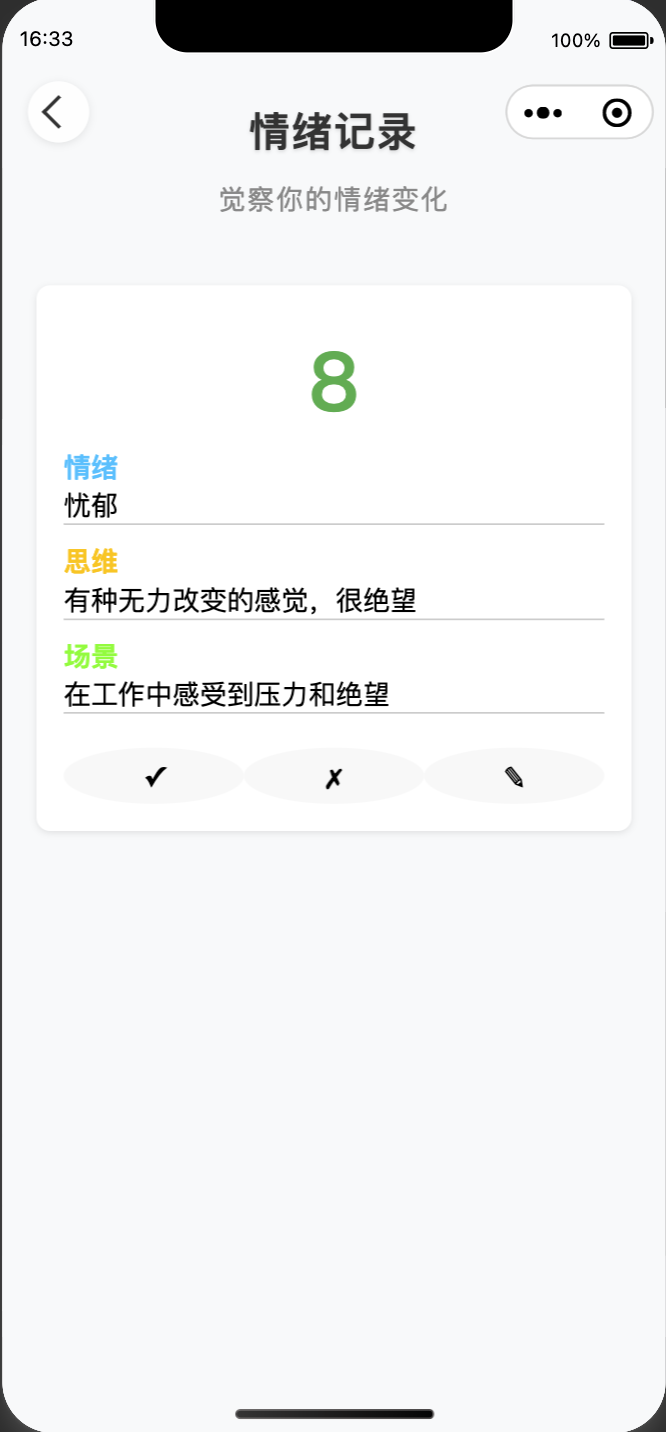
\includegraphics[width=0.48\linewidth]{figs/evidence-based content-and-feedback.jpg.jpg} \hfill
  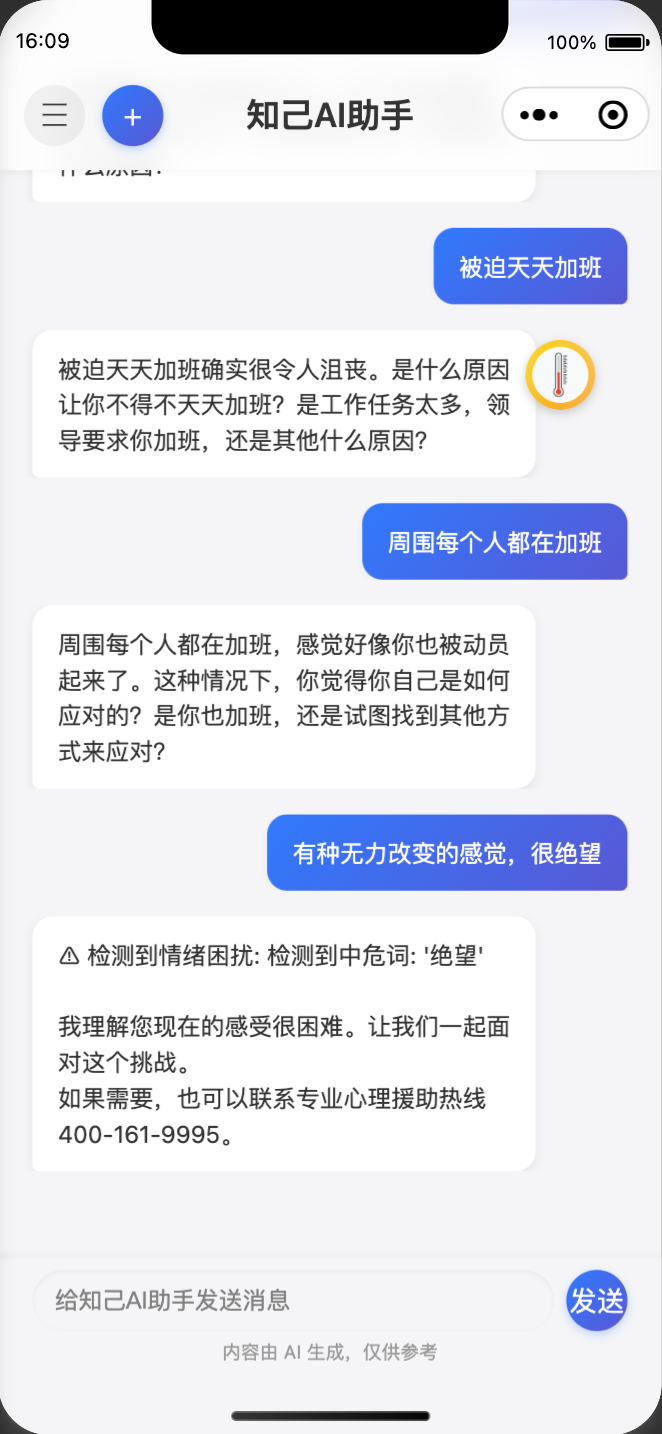
\includegraphics[width=0.48\linewidth]{figs/Crisis-management.jpg}
  \caption{
(a) Evidence-based content and feedback: The system presents user input in a structured manner as emotion intensity (8/10), type (depression), thinking content ("feeling powerless to change"), and triggering scenario ("feeling pressure at work"), with confirmation/editing buttons provided at the bottom; 
(b) Crisis management: After a user expresses work pressure ("forced to work overtime every day"), the AI helps the user perceive their emotions through questioning, and automatically provides psychological assistance hotline 400-161-9995 when it detects medium risk words such as "despair"
}
  \label{fig:illustrative-examples}
\end{figure}

\paragraph{Illustrative Examples}

\begin{itemize}
    \item \textbf{Evidence-based content and feedback:} As figure~\ref{fig:illustrative-examples}(a) illustrated, when a user expresses distress, the agent performs mood analysis and event extraction, presenting results as structured cards (e.g., mood intensity, category, cognitive appraisal, and triggering event). The user can edit or confirm these results, ensuring that the final record is both evidence-based and user-validated.
    \item \textbf{Crisis management:} As figure~\ref{fig:illustrative-examples}(b) illustrated, If the user input contains high-risk keywords (e.g., expressions of suicidal ideation), the agent immediately outputs a crisis intervention message and provides a psychological help hotline, in accordance with safety protocols.
\end{itemize}

Overall, the Introspection Agent demonstrates strong coverage of core FAITA-MENTAL domains related to evidence-based practice, personalization, interactivity, transparency, and safety. However, future work is needed to enhance user retention, autonomy, privacy, empowerment, and inclusivity.

